\documentclass[9pt]{IEEEtran}

\usepackage[english]{babel}
\usepackage{graphicx}
\usepackage{epstopdf}
\usepackage{fancyhdr}
\usepackage{amsmath}
\usepackage{amsthm}
\usepackage{amssymb}
\usepackage{url}
\usepackage{array}
\usepackage{textcomp}
\usepackage{listings}
\usepackage{hyperref}
\usepackage{xcolor}
\usepackage{colortbl}
\usepackage{float}
\usepackage{gensymb}
\usepackage{longtable}
\usepackage{supertabular}
\usepackage{multicol}

\usepackage[utf8x]{inputenc}

\usepackage[T1]{fontenc}
\usepackage{lmodern}{}
\input{glyphtounicode}
\pdfgentounicode=1

\graphicspath{{./figures/}}
\DeclareGraphicsExtensions{.pdf,.png,.jpg,.eps}

% correct bad hyphenation here
\hyphenation{op-tical net-works semi-conduc-tor trig-gs}

% ============================================================================================

\title{\vspace{0ex}
Optical flow}

\author{Marko Medved\vspace{-4.0ex}}

% ============================================================================================

\begin{document}

\maketitle

\section{Introduction}
In this assignment, we implemented the Lucas-Kanade and Horn-Schunck methods to estimate optical flow,
 which describes motion between video frames. We tested different parameters to determine the best settings
  for various scenarios. To improve the Lucas-Kanade method, we introduced a reliability criterion and 
  implemented a pyramidal structure.

\section{Experiments}
To begin, we present some implementation details that differ slightly from the explicit instructions
 for both methods. Gaussian smoothing was applied when calculating the time derivative in both methods.
In the Lucas-Kanade method, if the matrix used to compute flow at a given pixel was singular, the 
calculation was omitted, and a flow of 0 was assigned.
For the Horn-Schunck method, convergence was determined using the following equation: \[
\frac{\sum\limits_{\text{All pixels}} \left( (u - u_{\text{previous}})^2 + (v - v_{\text{previous}})^2 \right)}{\text{height} \times \text{width}}
\] where the u and v represent the flow in each pixel. The threshold of convergence is set 
to 1e-7. 

\subsection{Random noise evaluation}
First, the two methods were evaluated on random noise images, with the second image rotated by 1 degree 
to simulate motion. As shown in Figure~\ref{fig:LK_noise}, the Horn-Schunck method outperforms 
Lucas-Kanade, particularly along the edges where motion is faster. This result is expected since the 
Lucas-Kanade method assumes small motions.

\begin{figure}[h]
    \centering
    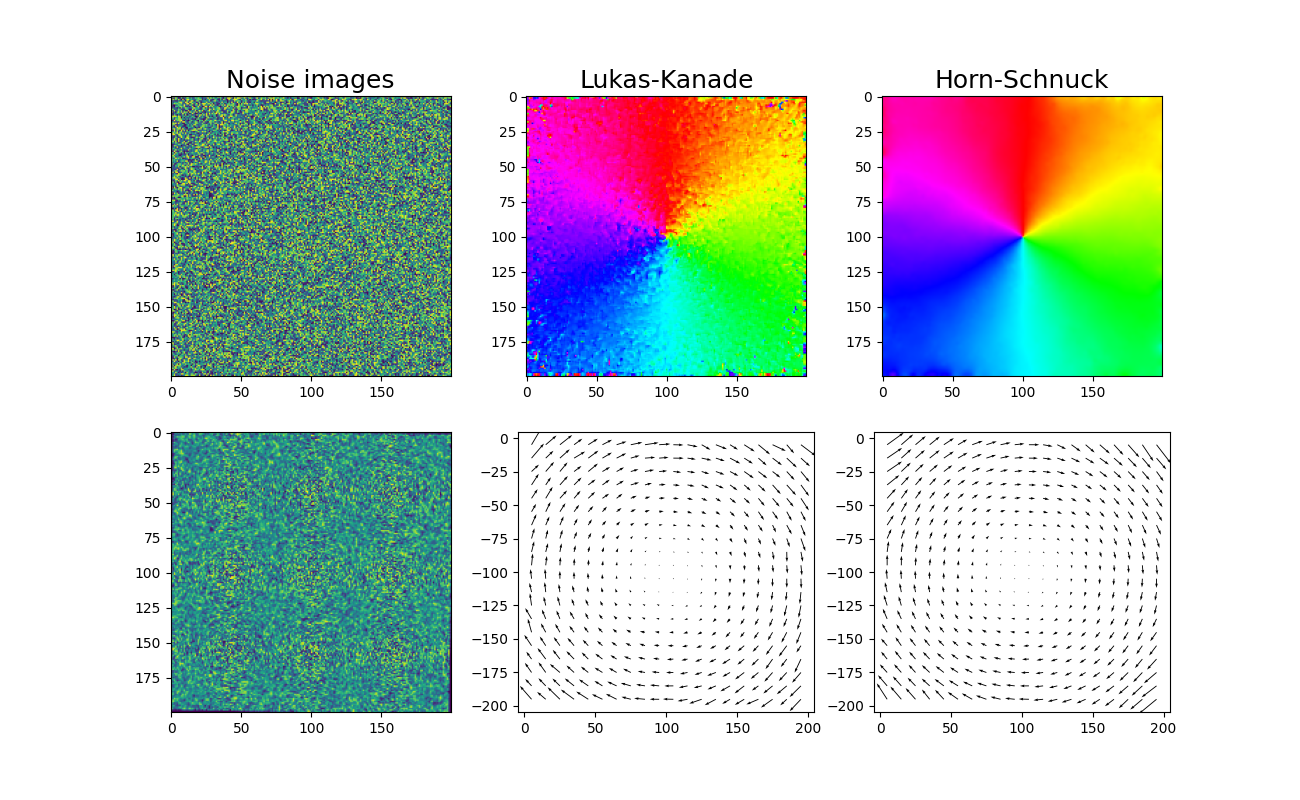
\includegraphics[width=0.8\columnwidth]{figures/noise.png}
    \caption{Comparison of Lukas-Kanade and Horn-Schnuck methods on real world examples.}
    \label{fig:LK_noise}
\end{figure}

\subsection{Testing the methods on real world examples.}

After testing on synthetic images, the methods were evaluated on real-world examples. As seen in 
Figure~\ref{fig:images}, the Horn-Schunck method generally produces a smooth flow field, with 
direction errors mainly occurring in areas with fine details, such as the trees in example 2.

The Lucas-Kanade method, however, struggles to capture motion direction in certain areas across all
 three examples. This is expected, as it tends to fail when the eigenvalues of the flow calculation
  matrix are both small or when their ratio is too large. The first issue arises when gradients in a 
  region have small magnitudes, as seen in example 2 (background sky) and example 3 (background wall). 
  The second issue occurs in edge-like structures, where the gradient is strong in only one direction. 
  An instance of this is in the third image, where the flow along the edges of the wardrobes appears
   entirely vertical.

 \begin{figure}[h]
    \centering
    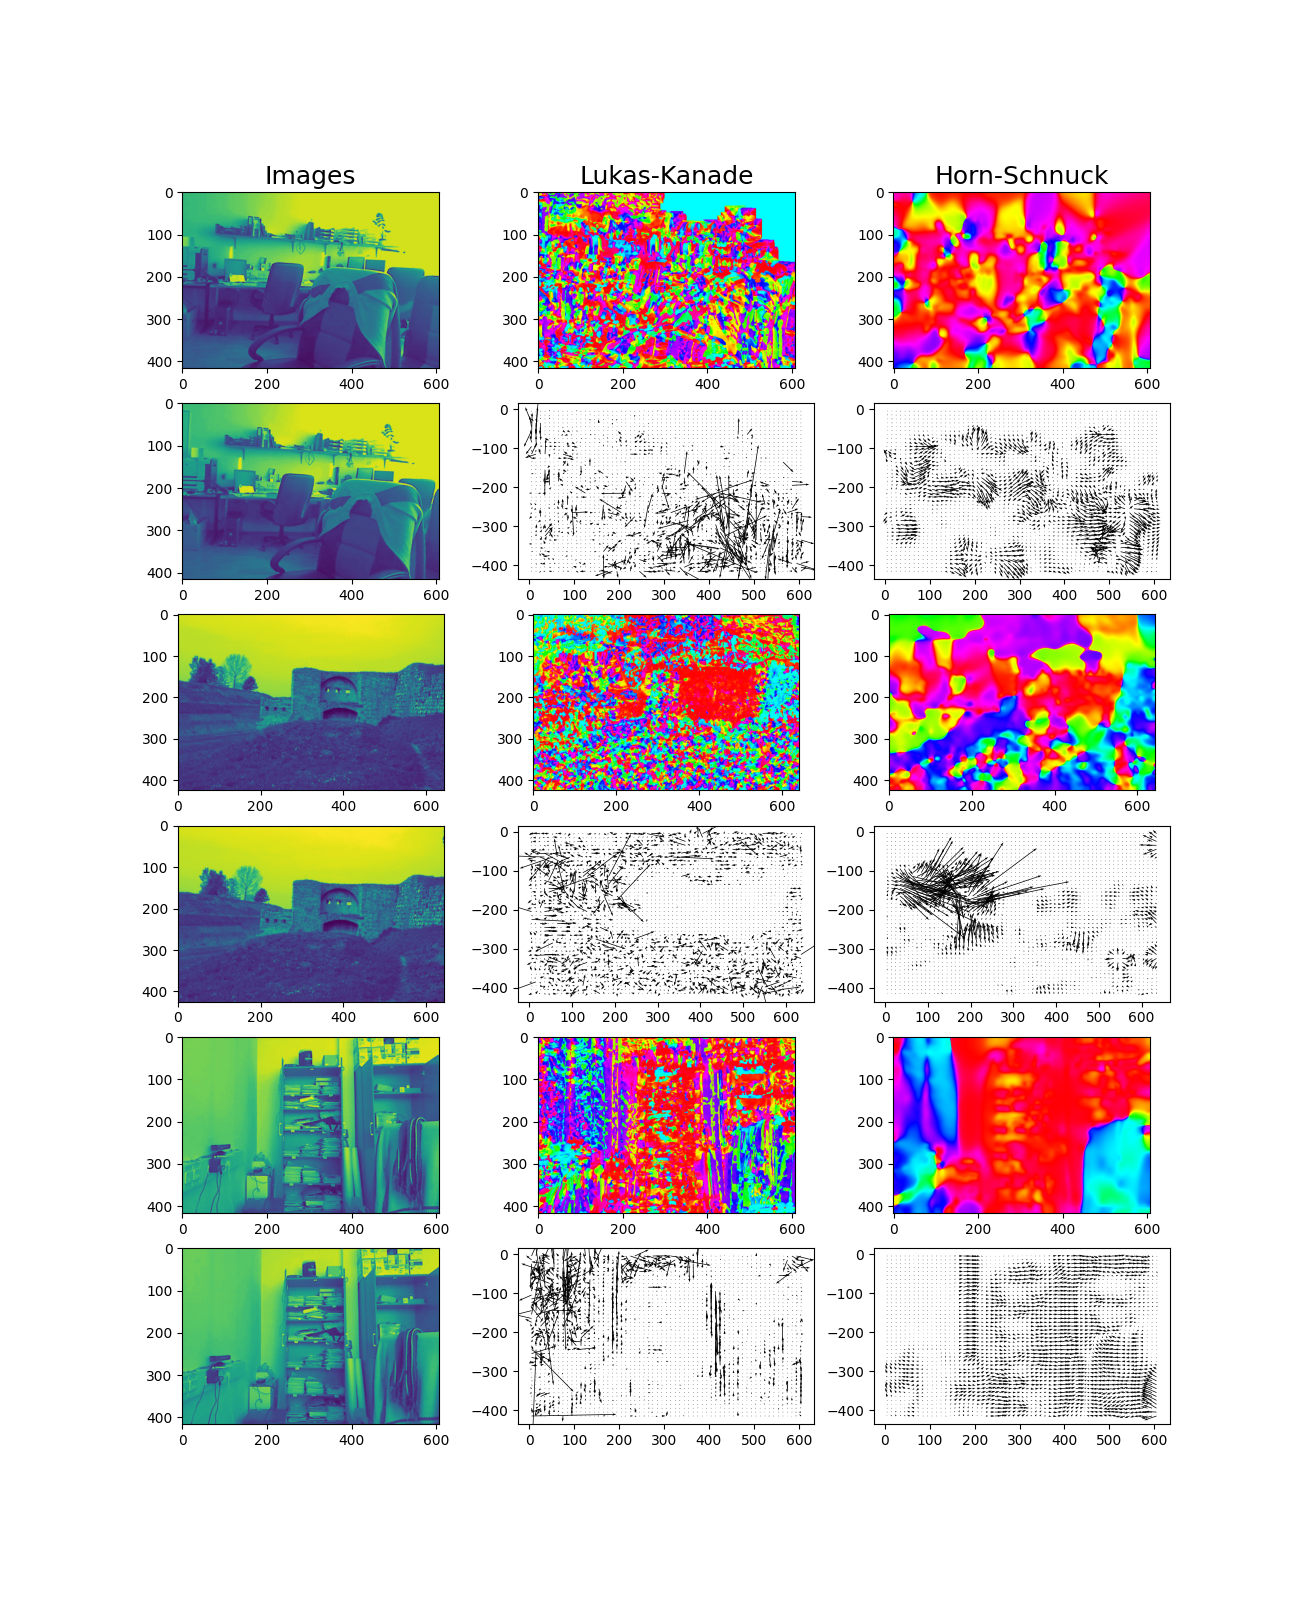
\includegraphics[width=1\columnwidth]{figures/images_base.png}
    \caption{Comparison of Lukas-Kanade and Horn-Schnuck methods on real world examples.}
    \label{fig:images}
\end{figure}

\subsection{Lukas-Kanade method reliability}
To address some of the previously mentioned issues with the Lucas-Kanade method, we utilized a
 technique to estimate the reliability of the optical flow at each pixel. While reliability 
 could be assessed by computing eigenvalues, this approach is computationally expensive. Instead, 
 we used the more efficient Harris corner detection method, which identifies regions where eigenvalues 
 are strong in both directions.

As shown in Figure~\ref{fig:harris}, this enhancement effectively reduces noise in uniform areas, 
such as the top-left wall in the image, and improves the flow direction near edges.

\begin{figure}[h]
    \centering
    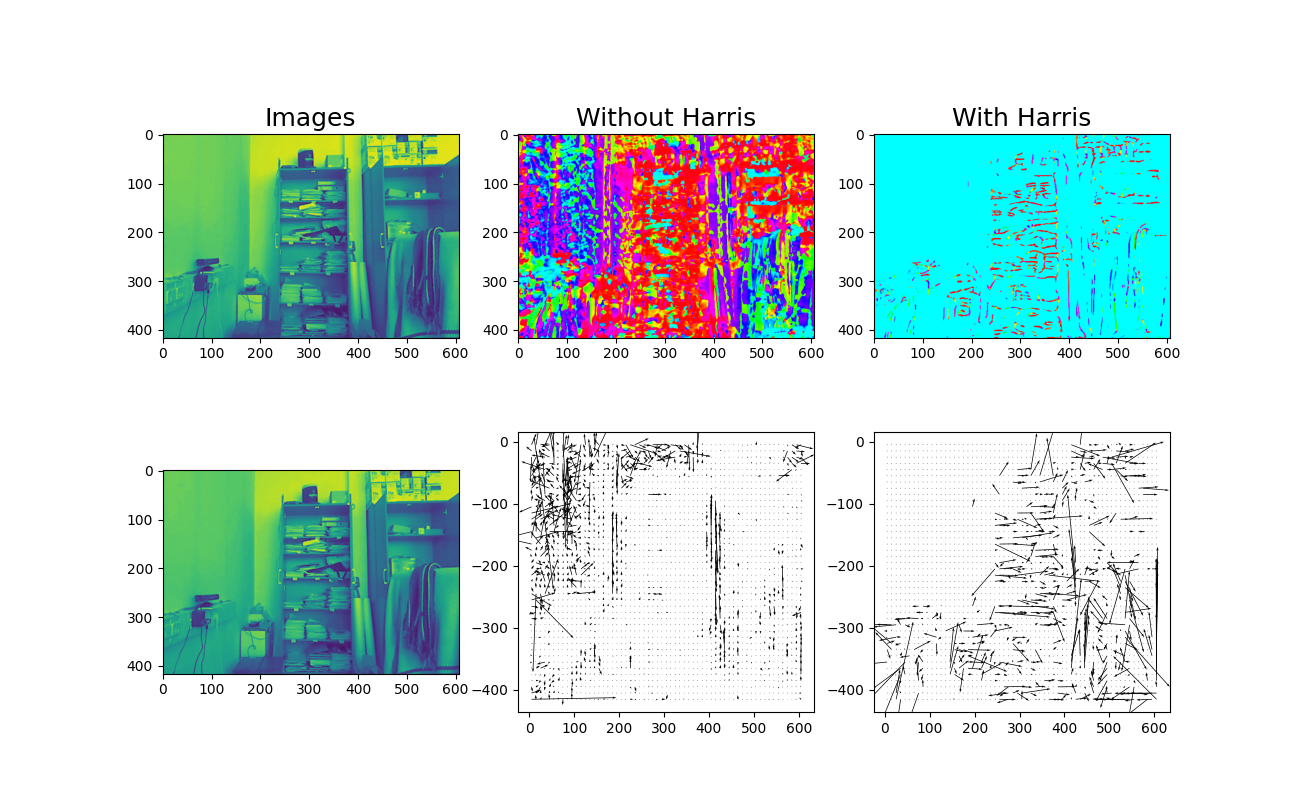
\includegraphics[width=1\columnwidth]{figures/harris_addition.png}
    \caption{Comparison of optical flow with and without the addition of Harris corner detection.}
    \label{fig:harris}
\end{figure}

\subsection{Parameter tuning}
Both methods use the sigma parameter, which controls the Gaussian filters applied for computing image 
derivatives and smoothing. This parameter was set to 1/170 of the image width to ensure it scales with 
image size.

The Lucas-Kanade method also relies on the N parameter, which defines the neighborhood size. As 
shown in Figure~\ref{fig:Lk_params}, a larger neighborhood results in a smoother flow field. However, 
increasing the neighborhood size reduces the ability to detect movement in smaller or more distant objects.

\begin{figure}[h]
    \centering
    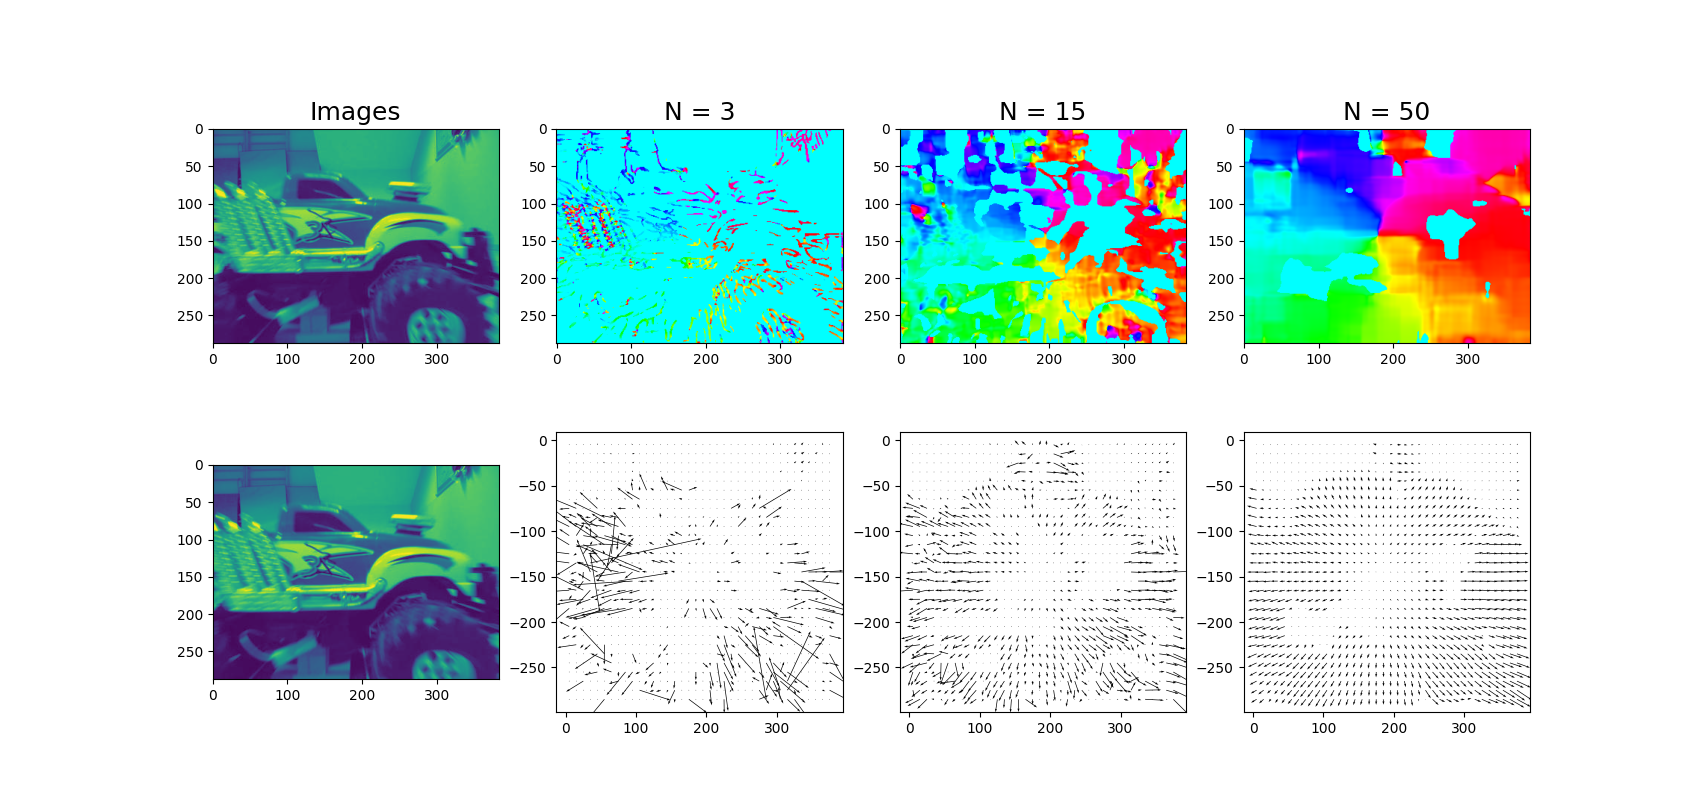
\includegraphics[width=1\columnwidth]{figures/LK_params.png}
    \caption{Comparison of optical flow using Lukas-Kanade with different sizes of neighbourhoods.}
    \label{fig:Lk_params}
\end{figure}

The Horn-Schunck method includes a lambda parameter, which controls the importance of the flow smoothness 
term, as well as the number of iterations, which only needs to be set high enough for the method to 
converge.
As shown in Figure~\ref{fig:HS_params}, a smaller lambda results in a less smooth flow field. However, 
if lambda is too large, some regions may lack a flow field entirely because too little emphasis is placed 
on color constancy and small motion errors. Therefore, in most cases, choosing a lambda between 0.1 and 1
 provides a good balance.


 \begin{figure}[h]
    \centering
    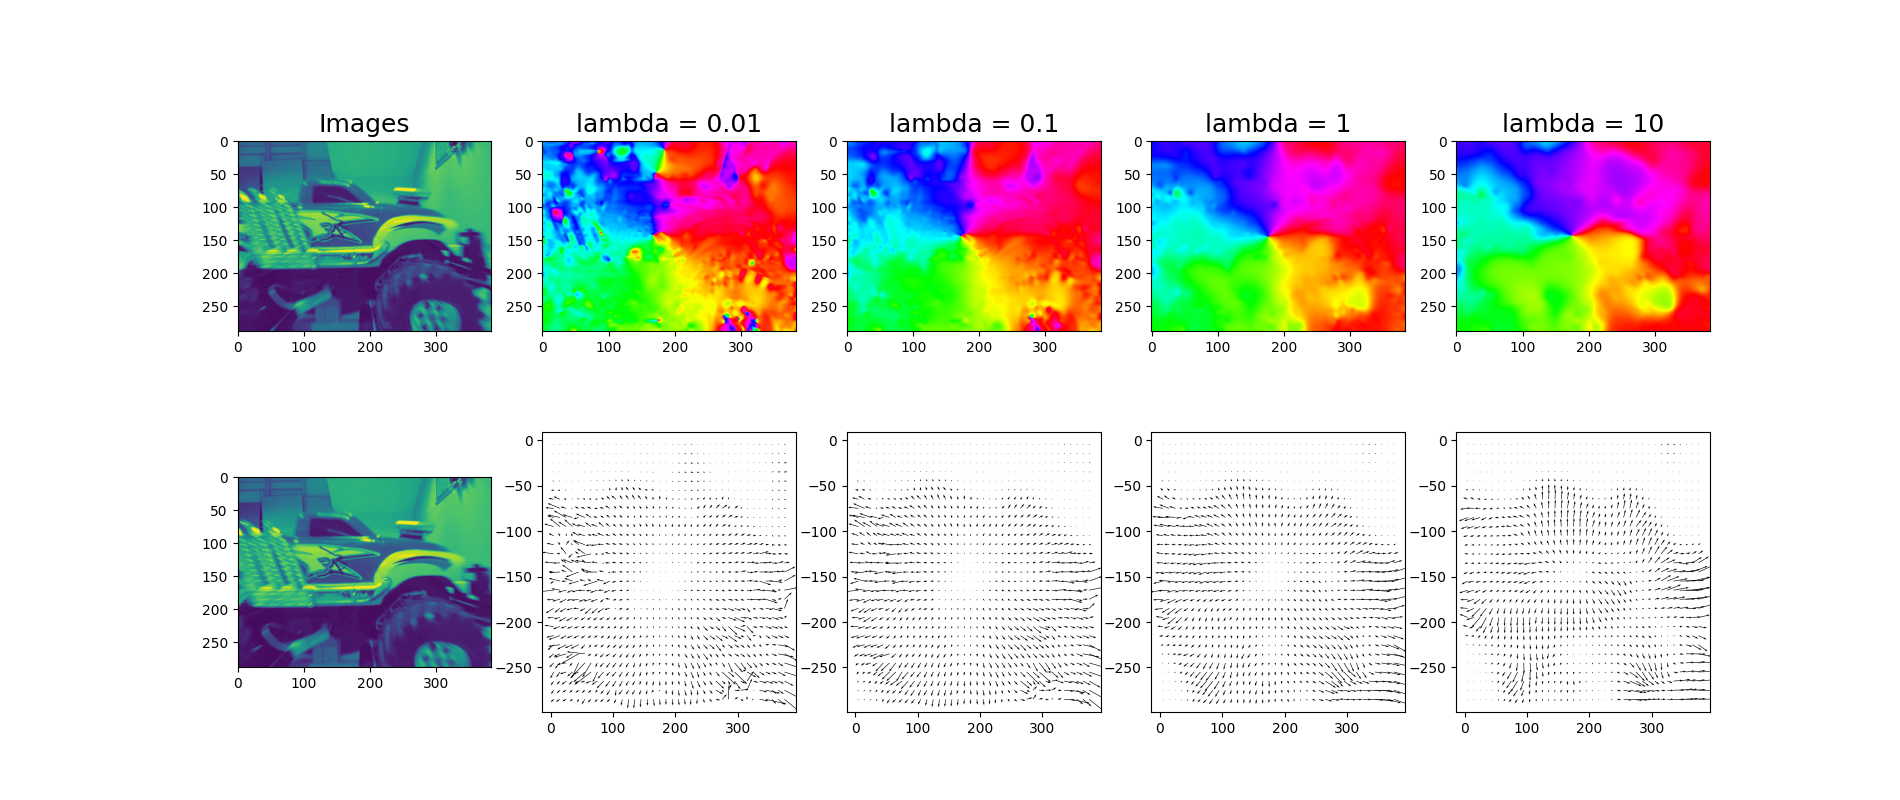
\includegraphics[width=1\columnwidth]{figures/HS_params.png}
    \caption{Comparison of optical flow using Horn-Schnuck with different weights on the smoothness error.}
    \label{fig:HS_params}
\end{figure}

\subsection{Time measurement}
While the Horn-Schunck method generally produces better results, it is significantly more time-consuming. 
We tested both methods on three different pairs of images and calculated their average runtime, as shown 
in Table~\ref{tab:time}. The measurements were performed 10 times and then averaged.

We also evaluated the Horn-Schunck method with Lucas-Kanade initialization. When the Lucas-Kanade 
neighborhood size was set to a large value (e.g., 50), there was a notable improvement in time efficiency, 
as shown in Table~\ref{tab:time}. However, using a smaller neighborhood (e.g., 3) resulted in slower 
convergence than the base Horn-Schunck method.
\begin{table}[h]
    \centering
    \begin{tabular}{c|c}
        \textbf{Method} & \textbf{Average time[s]} \\
        \hline
        Lukas-Kanade & 0.0310 $\pm$ 0.0001 \\
        Horn-Schnuck & 6.55 $\pm$ 0.02\\
        Horn-Schnuck (Lukas-Kanade initialization) & 4.27 $\pm$ 0.01  \\
    \end{tabular}
    \caption{Comparison of time-consumption for different methods}
    \label{tab:time}
\end{table}

\subsection{Pyramidal Lucas-Kanade}
We implemented the pyramidal version of the Lucas-Kanade method. Images that were at least 4 times 
the size of the neighborhood (we used a neighborhood size of 15) were input into the pyramid.
As shown in Figure~\ref{fig:pyramidal}, the pyramidal structure produces a smooth optical flow, 
even when the image has a highly diverse background, as in this example. The advantage of the pyramidal
 structure is that it can capture both small and large movements. Additionally, we observed that applying 
 the method multiple times at each level slightly improved the flow direction in the bottom-right area

\begin{figure}[h]
    \centering
    \includegraphics[width=1\columnwidth]{figures/Pyramidal.png}
    \caption{Comparison of the base Lukas-Kanade method with its pyramidal alternative, without and with 7 repetitions at each resolution.}
    \label{fig:pyramidal}
\end{figure}

\section{Conclusion}

The experimentation showed that the Horn-Schunck method generally performs better than the Lucas-Kanade
 method. However, it is significantly slower, which is a critical factor for many motion tracking 
 applications. We demonstrated that the Lucas-Kanade method can be improved by introducing a reliability 
 criterion for flow estimation and incorporating a pyramidal structure.

\bibliographystyle{IEEEtran}
\bibliography{bibliography}

\end{document}
